\documentclass[a4paper,14pt]{extreport}
	\usepackage[left=1.5cm,right=1.5cm,
	    top=1.5cm,bottom=2cm,bindingoffset=0cm]{geometry}
	\usepackage{scrextend}
	\usepackage[T1,T2A]{fontenc}
	\usepackage[utf8]{inputenc}
	\usepackage[english,russian,ukrainian]{babel}
	\usepackage{tabularx}
	\usepackage{pgfplots}
	\usepackage{amssymb}
	\linespread{1.5}
	\usepackage{color}
	\usepackage{amsmath}
	\usepackage{mathrsfs}
	\usepackage{listings}
	\usepackage{graphicx}
	\graphicspath{ {./images/} }
	\usepackage{lipsum}
	\usepackage{xcolor}
	\usepackage{hyperref}
	\usepackage{tcolorbox}
	\usepackage{tikz}
	\usepackage[framemethod=TikZ]{mdframed}
	\usepackage{wrapfig,boxedminipage,lipsum}
	\mdfdefinestyle{MyFrame}{%
	linecolor=blue,outerlinewidth=2pt,roundcorner=20pt,innertopmargin=\baselineskip,innerbottommargin=\baselineskip,innerrightmargin=20pt,innerleftmargin=20pt,backgroundcolor=gray!50!white}
	 \usepackage{csvsimple}
	 \usepackage{supertabular}
	\usepackage{pdflscape}
	\usepackage{fancyvrb}
	%\usepackage{comment}
	\usepackage{array,tabularx}
	\usepackage{colortbl}
	\usepackage{fp}

	\usepackage{varwidth}
	\tcbuselibrary{skins}
	\usepackage{fancybox}


	\usepackage{tikz}
	\usepackage[framemethod=TikZ]{mdframed}
	\usepackage{xcolor}
	\usetikzlibrary{calc}
	\makeatletter
	\newlength{\mylength}
	\xdef\CircleFactor{1.1}
	\setlength\mylength{\dimexpr\f@size pt}
	\newsavebox{\mybox}
	\newcommand*\circled[2][draw=blue]{\savebox\mybox{\vbox{\vphantom{WL1/}#1}}\setlength\mylength{\dimexpr\CircleFactor\dimexpr\ht\mybox+\dp\mybox\relax\relax}\tikzset{mystyle/.style={circle,#1,minimum height={\mylength}}}
	\tikz[baseline=(char.base)]
	\node[mystyle] (char) {#2};}
	\makeatother

	\definecolor{ggreen}{rgb}{0.4,1,0}
	\definecolor{rred}{rgb}{1,0.1,0.1}
	\definecolor{amber}{rgb}{1.0, 0.75, 0.0}
	\definecolor{babyblue}{rgb}{0.54, 0.81, 0.94}
	\definecolor{amethyst}{rgb}{0.6, 0.4, 0.8}

	\usepackage{float}
	\usepackage{wrapfig}
	\usepackage{framed}
	%for nice Code{
	\lstdefinestyle{customc}{
	  belowcaptionskip=1\baselineskip,
	  breaklines=true,
	  frame=L,
	  xleftmargin=\parindent,
	  language=C,
	  showstringspaces=false,
	  basicstyle=\small\ttfamily,
	  keywordstyle=\bfseries\color{green!40!black},
	  commentstyle=\itshape\color{purple!40!black},
	  identifierstyle=\color{blue},
	  stringstyle=\color{orange},
	}
	\lstset{escapechar=@,style=customc}
%}


\begin{document}
\pagecolor{white}

%----------------------------------------1
\newtcbox{\xmybox}[1][red]{on line, arc=7pt,colback=#1!10!white,colframe=#1!50!black, before upper={\rule[-3pt]{0pt}{10pt}},boxrule=1pt, boxsep=0pt,left=6pt,right=6pt,top=2pt,bottom=2pt}



\begin{titlepage}
	\begin{center}
	\large
	Національний технічний університет України \\ "Київський політехнічний інститут імені Ігоря Сікорського"


	Факультет Електроніки

	Кафедра мікроелектроніки
	\vfill

	\textsc{ЗВІТ}\\

	{\Large Про виконання лабораторної роботи №3\\
	з дисципліни: «Твердотільна електроніки-2»\\[1cm]

	«Дослідження поверхні напівпровідника методом вольт-фарадних характеристик МДН-структури» \\

	}
	\bigskip
	\end{center}
	\vfill

	\newlength{\ML}
	\settowidth{\ML}{«\underline{\hspace{0.4cm}}» \underline{\hspace{2cm}}}
	\hfill
	\begin{minipage}{1\textwidth}
	Виконавець:\\
	Студент 3-го курсу \hspace{4cm} $\underset{\text{(підпис)}}{\underline{\hspace{0.2\textwidth}}}$  \hspace{1cm}Б.\,П.~Фіцай\\
	\vspace{1cm}

	Превірив: \hspace{6.1cm} $\underset{\text{(підпис)}}{\underline{\hspace{0.2\textwidth}}}$  \hspace{1cm}Л.\,М.~Королевич\\

	\end{minipage}

	\vfill

	\begin{center}
	2021
	\end{center}
\end{titlepage}
%---------------------------------------------------------------------------------------------------------------------------------------------------------------------------------
\newpage
\setcounter{page}{2}



\begin{center}1. МЕТА РОБОТИ\\ \end{center}

Дослідження величини, природи та стабільності заряду поверхневих
станів напівпровідника з допомогою вольт-фарадних характеристик ємності
структури метал-діелектрик-напівпровідник (МДН).

\begin{center}2. ЗАВДАННЯ\\ \end{center}

	1. Скласти схему для вимірювання ємності МДН-структури.\\

	2. Виконати вимірювання вольт-фарадної характеристики – залежності 
	ємності конденсатора МДН-структури від напруги зміщення. Діапазон напруг 
	від -20 В до +20 В. Частота вимірювального сигналу 1...2 МГц.\\

	3. Провести «вольт-температурні (В-Т) випробування» МДН-структури 
	при додатній та (або) при від’ємній полярностях постійної напруги., 
	прикладеної під час витримки при високій температурі.\\

	4. Побудувати зняті графіки вольт-фарадних (В-Ф) характеристик на 
	одному малюнку.\\

	5. Визначити за видом знятої вольт-фарадної характеристики тип 
	провідності напівпровідникової основи мікросхеми.\\

	6. Розрахувати із первинної В-Ф-характеристики величину, густину та 
	полярність заряду поверхневих станів.\\

	7. Розрахувати зміну заряду після «В-Т-випробувань» і пояснити природу 
	походження та причину нестабільності заряду поверхневих станів в 
	дослідженій МДН структури.



\newpage
\begin{center}СХЕМА ДОСЛІДЖЕННЯ\\ \end{center}

\begin{figure}[h]
\center{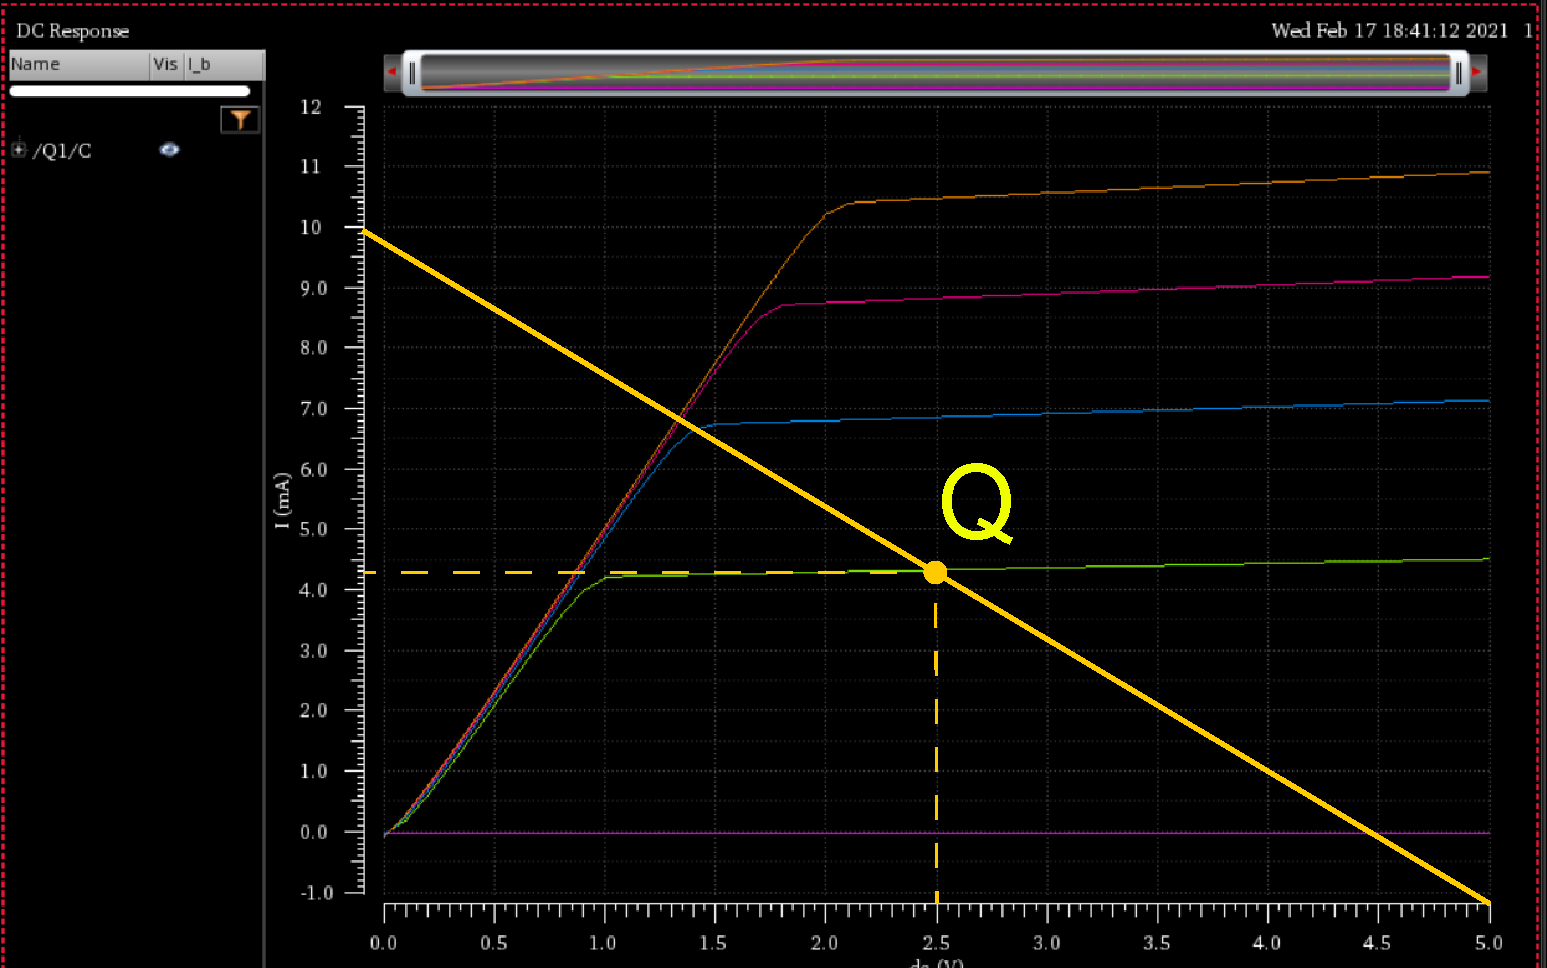
\includegraphics[width=0.8\linewidth]{1.png}}
\caption{Електрична схема установки дослідження вольт-фарадних 
характеристик}
\label{ris1}
\end{figure}




\clearpage
\begin{center}Таблиці\\ \end{center}


\begin{figure}[h]
\center{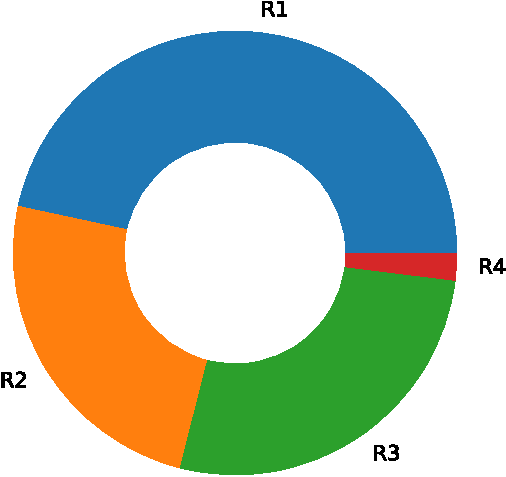
\includegraphics[width=0.8\linewidth]{2.png}}
\caption{Табл. 1 Вимірювання Вольт-Фарадних характеристик МДН-структури
	Умови вимірювань: $C_0$=370пФ; $F_0$=1,44МГц; $S_{\text{мдн}}$=1 мм$^2$. $\triangle C$ = 0,1 пФ; $\triangle U$ = 5 мВ. $\varepsilon$ = 3.9}
\label{ris2}
\end{figure}


%---------------------------------------------------------------------------------------------------------------------------------------------------------------------------------

\newpage
\begin{figure}[h]
\center{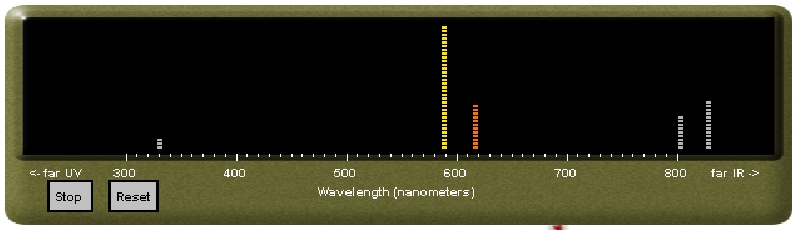
\includegraphics[width=0.7\linewidth]{3.png}}
\caption{вольт-фарадні характеристики нашої МДН-структури}
\label{ris3}
\end{figure}



\clearpage
Висновок: \\ 

	В даній лабораторній роботі було досліджено ємності структури МДН за допомогою отриманих вольт-фарадних характеристик. В ході виконання лабораторної роботі було виявлено, що при змiнi температури напiвпровiдника змiнюється об’ємне положення рiвня Фермi. МДН структура, що  досліджувалася, створена на основі кремнію n–типу, що видно з кута нахилу Вольт-Фарадної характеристики до осі напруги. Залежність відповідає теоретичній: має дві ділянки з постійним значенням, між якими – різке зростання від мінімального значення до максимального. Пояснюється така особливість вольт-фарадної характеристики тим, що за додатних напруг, напівпровідник несе нульовий вклад у сумарну ємність структури. При зменшенні напруги на затворі відбувається зміщення зарядів і з’являється бар'єрна ємність, внаслідок чого сумарна ємність зменшується.





\end{document}
